\chapter{Reconstruction expérimentale d'événements \ttbar}

Les \cref{chap:zprime,chap:higgs} sont consacrés à la recherche de nouvelle physique dans le spectre de masse invariante de paire \ttbar. Avant de pouvoir chercher de quelconques déviation dans le spectre de masse, il faut être capable de reconstruire la masse invariante du système \ttbar. On présente dans ce chapitre les techniques de reconstruction de la masse invariante.

\section{Masse invariante}

La masse invariante est un invariant relativiste définie par
\begin{align*}
  m^2 &= E^2 - \norm{\vec{p}}^2
\end{align*}

Lorsqu'une particule de masse $m$ se désintègre, $X \rightarrow A + B$ la masse invariante est conservée ($m_X = m_{A + B}$). La masse invariante du système A + B est définie par :
\begin{align*}
  m_{A + B}^2 &= \left( E_A + E_B \right)^2 - \norm{ \vec{p}_A + \vec{p}_B }^2
\end{align*}

Cette relation est aisément extensible à un système de $N$ particules. Dans le cas de particule sans masse, ou hautement relativiste ($E \gg m$, toujours le cas au LHC), on peut exprimer la masse invariante en fonction des variables angulaires des particules :
\begin{align*}
  m_{A + B}^2 &= 2 p_T^A p_T^B \left( \cosh{\left( \eta_A - \eta_B \right)} - \cos{\left( \phi_A - \phi_B \right)} \right)
\end{align*}

En utilisant le quadrivecteur énergie-impulsion ($p = \left(E,\,\vec{p}\right)$), la masse invariante est simplement définie comme la norme de $p$ :
\begin{align*}
  m &= \norm{p}
\end{align*}

\subsection{Masse invariante du système \ttbar}

Concentrons nous uniquement sur le canal semi-leptonique, c'est-à-dire un quark top qui se désintègrent en \Plepton{}\Pneutrino{}\Pbottom, et le deuxième en \Pbottom{}\Pquark{}\APquark (voir \cref{fig:top_pair_decay_semileptonic}). Toutes les particules peuvent être reconstruites, excepté le neutrino. En effet, n'interagissant que très faiblement avec la matière, les neutrinos traversent le détecteur sans laisser de dépôts dans les sous-détecteurs. Le seul moyen d'identifier les neutrinos est d'utiliser l'énergie transverse manquante. En faisant le bilan d'énergie de la collision dans le plan transverse, le neutrino apparait comme de l'énergie manquante. Dans le cas d'une désintégration \ttbar, on identifie donc l'énergie transverse manquante comme le neutrino.

Afin de reconstruire la masse invariante du système \ttbar, il faut être capable de reconstruire la cinématique de chaque produit de la désintégration. On peut ensuite reconstruire la masse invariante \ttbar :
\begin{align} \label{eq:invariant_mass_tt}
  m_{\ttbar} &= \norm{ p_{\Plepton} + p_{\Pneutrino} + p_{\Pquark} + p_{\APquark} + p_{\Pbottom}^{\text{hadronique}} + p_{\Pbottom}^\text{leptonique} }
\end{align}

Deux problèmes majeures se posent :
\begin{itemize}
    \item 4 jets composent l'état final d'une désintégration \ttbar. Il faut donc être capable de correctement identifier ces jets parmi les nombreux jets de \pu dans l'événement. Pour cela, diverses techniques peuvent être employées, décrites plus loin dans ce chapitre.
    \item L'énergie transverse manquante est utilisée pour reconstruire le neutrino. Comme le bilan d'énergie ne peut être effectué que dans le plan transverse, seul l'impulsion transverse du neutrino est définie, c'est-à-dire $p_x$ et $p_y$. Il faut donc trouver un moyen de reconstruire $p_z$ qui sera utilisé dans le calcul de la masse invariante \ttbar. C'est l'objet de la \cref{sec:neutrino}.
\end{itemize}

Une fois ces problèmes surmontés, il est possible de reconstruire la masse invariante pour chaque événement. Il est ainsi possible d'obtenir un spectre de masse invariante.

\section{Reconstruction du neutrino} \label{sec:neutrino}

Comme on a vu précédemment, la présence d'un neutrino se caractérise par de l'énergie manquante. En considérant que la seule source d'énergie manquante dans l'événement, on a alors
\begin{align*}
  p_t^{\Pneutrino} &= \met
\end{align*}

Afin de reconstruire la masse invariante, il faut pouvoir reconstruire la composante longitudinale de l'impulsion transverse du neutrino. On sait que le neutrino émis vient obligatoirement de la désintégration d'un boson \PW en $\Plepton + \Pneutrino$. On peut déterminer la composante $p_z$ de l'impulsion du neutrino en utilisant comme contrainte la valeur de la masse du boson \PW ($m = \SI{80.385 \pm 0.015}{\GeV}$ \citep{pdg}). On a :
\begin{align*}
  m_{\PW}^2 &= \left( E_{\Pneutrino} + E_{\Plepton} \right)^2 - \norm{ \vec{p}_{\Pneutrino} + \vec{p}_{\Plepton} }^2 \\
  &= m_{\Plepton} + 2E_{\Pneutrino}E_{\Plepton} - 2 \vec{p}_{\Pneutrino} \cdot \vec{p}_{\Plepton}
\end{align*}

Après quelques calculs, on obtient une équation d'ordre 2 permettant de déterminer $p_z$ :
\begin{align*}
  a \, \left( p_z^{{\Pneutrino}} \right)^2 + b \, p_z^{{\Pneutrino}} + c &= 0
\end{align*}
avec
\begin{align*}
  a &= E_{\Plepton}^2 - \left( p_z^{{\Pneutrino}} \right)^2 \\
  b &= \left( m_{\Plepton}^2 - m_{\PW}^2 - 2 \left( p_x^{\Plepton} p_x^{\Pneutrino} + p_y^{\Plepton} p_y^{\Pneutrino} \right) \right) p_z^{\Plepton} \\
  c &= E_{\Plepton}^2 \left( p_z^{\Pneutrino} \right)^2 - \left( \frac{1}{2} \left( m_{\PW}^2 - m_{\Plepton}^2 \right) + p_x^{\Plepton} p_x^{\Pneutrino} + p_y^{\Plepton} p_y^{\Pneutrino} \right)^2
\end{align*}

\begin{figure}[tbp]
    \centering
    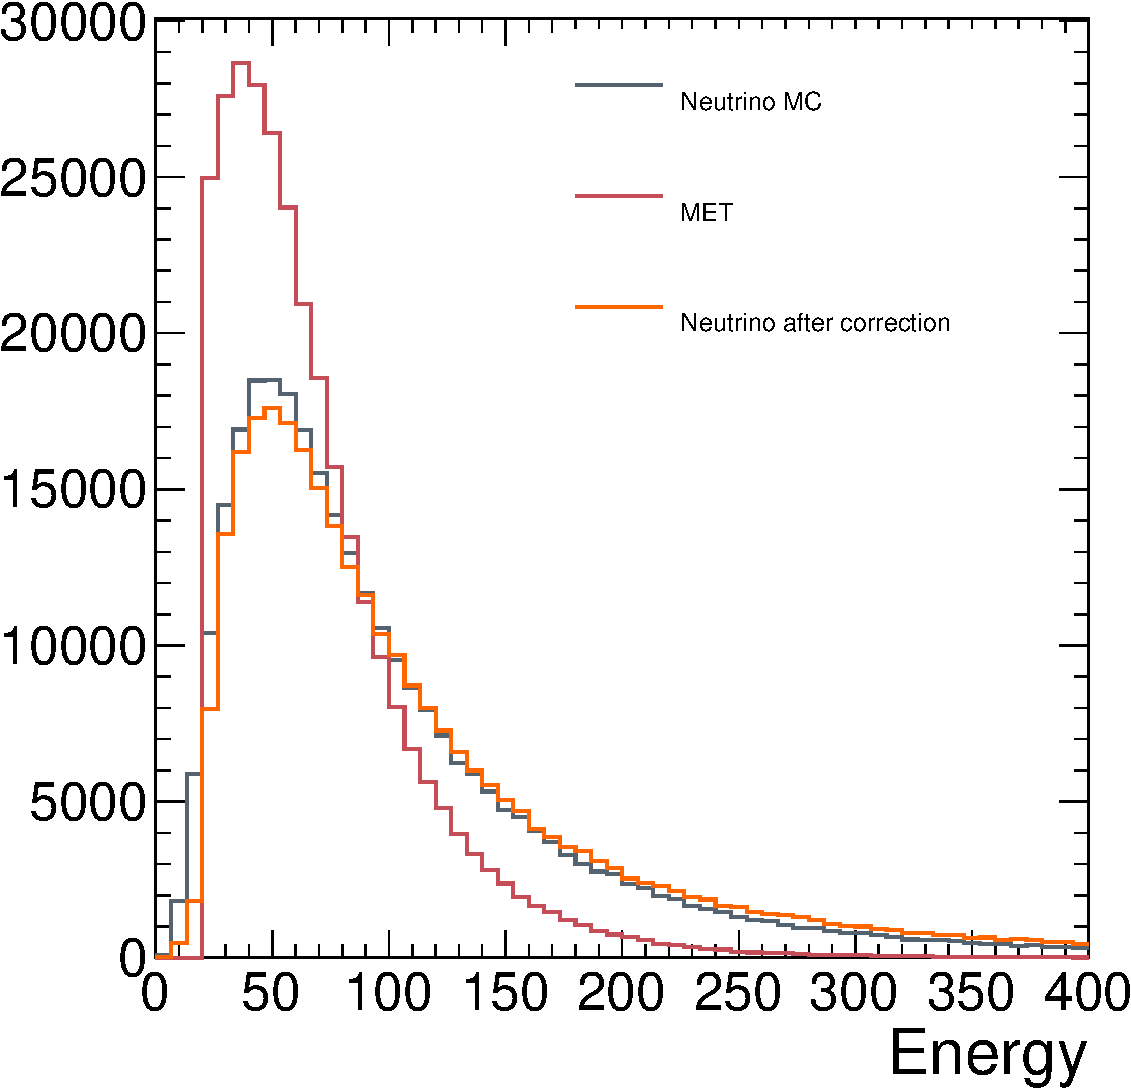
\includegraphics[width=0.55\textwidth]{chapitre6/figs/neutrino_energy/plot_met_energy.pdf}
    \caption{Effet de la reconstruction de la composante longitudinale du neutrino sur la mesure de l'énergie du neutrino sur des événements \ttbar simulés (en \textcolor{rouge_grandmere}{rouge}, avant reconstruction de $p_z$, en \textcolor{orange}{orange} après reconstruction). À titre de comparaison, l'énergie du neutrino au niveau générateur (en \textcolor{bleu_gris}{bleu}) est aussi tracée.}
    \label{fig:neutrino_correction}
\end{figure}

Dans \tilde\SI{16}{\%} des cas, cette équation n'a pas de solution réelle. Cela peut être le cas lorsque l'énergie transverse manquante est surestimée. Dans ce cas, on cherche une solution réelle en faisant varier $p_x^{\Pneutrino}$ et $p_y^{\Pneutrino}$ de façon identique et synchronisée jusqu'à obtenir une solution réelle.

Lorsque l'on obtient deux solutions réelles, le choix est fait en utilisant la contrainte de la masse du quark top. Le neutrino provient en effet de la cascade de désintégration $\Ptop \rightarrow \Pbottom \PW$, $\PW \rightarrow \Plepton \Pneutrino$. On retient la solution qui donne la masse invariante à trois corps entre le lepton, le neutrino et le jet \Pbottom leptonique la plus proche de la masse du quark top.

\medskip

On présente \cref{fig:neutrino_correction} l'effet de la reconstruction de la composante longitudinale sur la mesure de l'énergie du neutrino. Avant reconstruction, l'énergie du neutrino est clairement sous estimée. Une fois $p_z$ reconstruit, l'énergie du neutrino coïncide avec l'énergie du neutrino générée. On mesure ici toute l'importance de la reconstruction du neutrino sur la mesure de l'énergie, et donc sur la reconstruction de la masse invariante du système \ttbar.

\section{Méthodes d'appariement des jets}

Lors d'une désintégration \ttbar dans le canal semi-leptonique, 4 jets composent l'état final : 2 jets de \Pbottom, provenant de la désintégrations des deux quarks top, et deux jets de quark légers, provenant de la désintégration d'un des bosons \PW.

Le LHC est un collisionneur hadronique. De nombreux jets additionnels sont produits lors d'une collision, venant du \pu, de l'événement sous-jacent, de radiations de gluon, etc. Il faut donc un moyen d'identifier précisément les jets provenant de la désintégration \ttbar parmi tous les jets de l'événement. Deux méthodes sont étudiées dans cette section, la méthode de tri par $\chi^2$, et la méthode de tri par MVA (\emph{Multi-Variate Analysis}, analyse multi-variée).

\medskip

Ces deux méthodes sont utilisées après sélection. Cette sélection ne sera pas détaillée dans cette section, puisqu'elle est dépendante de l'analyse. Néanmoins, on sélectionne typiquement des événements ayant un seul lepton isolé (électron ou muon), et au moins 4 jets. Ces événements constitues la signature expérimentale d'une événement \ttbar, et sont appelés événements candidats \ttbar.

\subsection{Algorithme de tri par \texorpdfstring{$\chi^2$}{chi²}}

Pour chaque événement candidat \ttbar, parmi $N (\geq 4)$ jets sélectionnés, on distingue $\binom{N}{N - 4}$ sous-ensembles de 4 jets. Pour chaque sous ensemble, on compte 12 combinaisons possibles pour assigner les jets si l'on considère les jets provenant de la désintégration du \PW hadronique indiscernables.

\medskip

Afin de choisir la bonne combinaison, on minimise une variable de $\chi^2$, construite à partir de composantes qui permettent de discriminer entre les bonnes et les mauvaises combinaisons. Le $\chi^2$ total est donné par
\begin{align} \label{eq:chi2}
  \chi^2 &= \chi^2_{m_{\Ptop}^{\text{lept.}}} + \chi^2_{m_{\Ptop}^{\text{hadr.}}} + \chi^2_{m_{\PW}^{\text{hadr.}}} + \chi^2_{H_{T}^{\text{frac.}}}
\end{align}
où

\begin{align*}
  \chi^2_X &= \frac{\left( X_\text{mesuré} - X_\text{MC} \right)^2}{\sigma_\text{MC}^2}
\end{align*}
avec $X$ le discriminant considéré, $X_\text{mesuré}$ la valeur du discriminant mesurée, $X_\text{MC}$ la valeur la plus probable du discriminant déterminé sur la simulation et $\sigma_\text{MC}$ l'erreur sur la valeur la plus probable du discriminant.

Les discriminants formant le $\chi^2$ total sont :
\begin{itemize}
    \item $\chi^2_{m_{\Ptop}^{\text{lept.}}}$ : masse du quark top dans la branche leptonique. Des valeurs différentes sont utilisées pour les sélections avec un électron ou un muon.
    \item $\chi^2_{m_{\Ptop}^{\text{hadr.}}}$ : masse du quark top dans la branche hadronique.
    \item $\chi^2_{m_{\PW}^{\text{hadr.}}}$ : masse du boson \PW dans la branche hadronique.
    \item $\chi^2_{H_{T}^{\text{frac.}}}$ : $\sum\limits_i{p_T} / \sum\limits_j{p_T}$ où $i$ court sur les 4 jets considérés, et $j$ sur tous les jets sélectionnés.
\end{itemize}

\begin{figure}[p] \centering
    \subcaptionbox{}[0.41\textwidth]{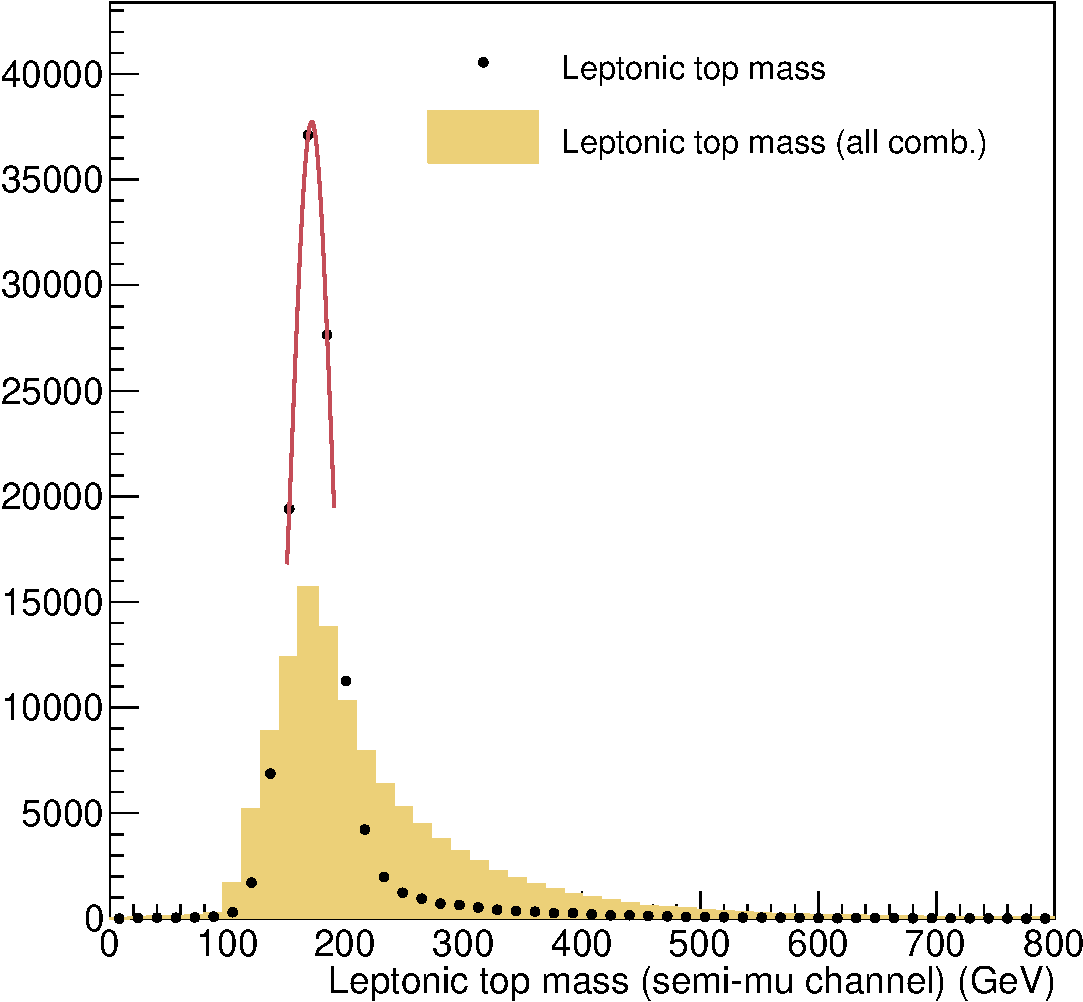
\includegraphics[width=0.41\textwidth]{chapitre6/figs/chi2/chi2_discrimant_combinations_leptonic_top_mass_mu.pdf}} \qquad
    \subcaptionbox{}[0.41\textwidth]{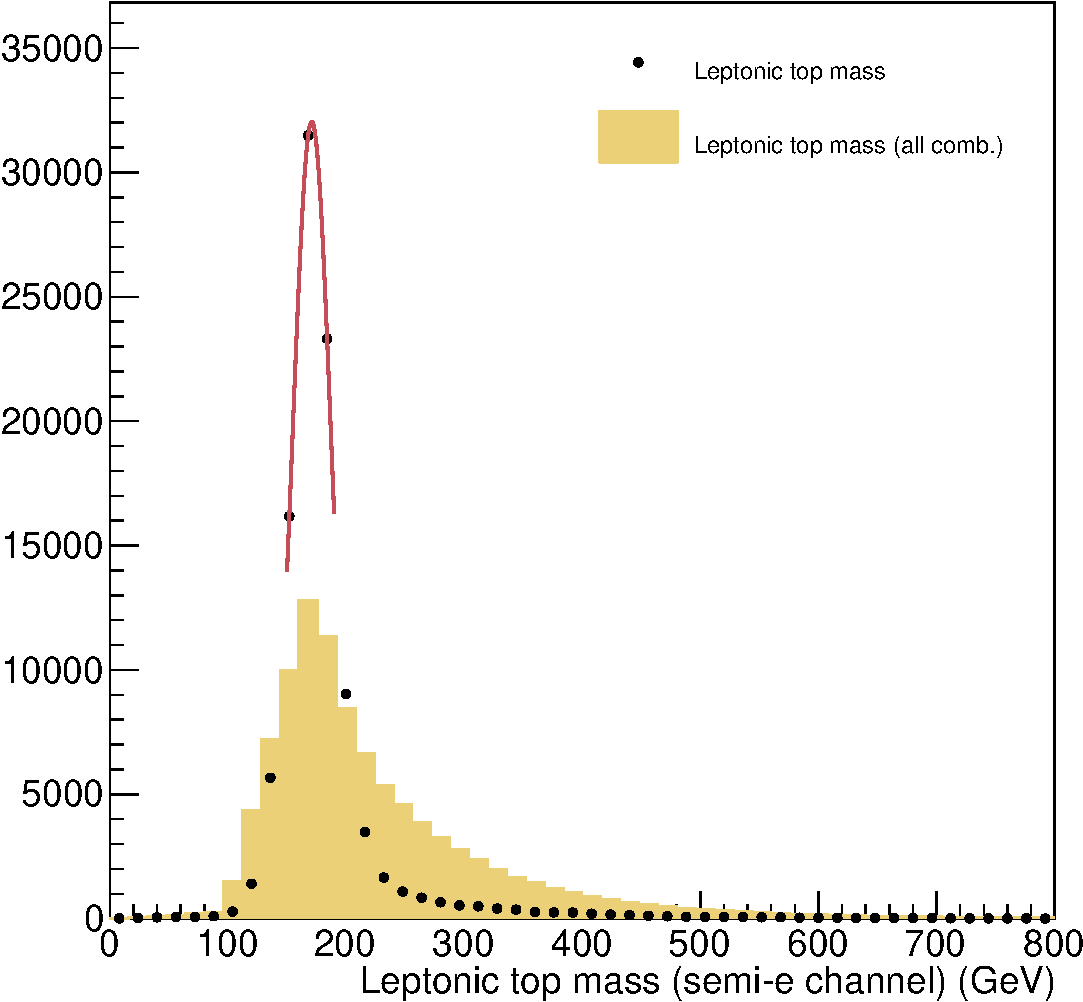
\includegraphics[width=0.41\textwidth]{chapitre6/figs/chi2/chi2_discrimant_combinations_leptonic_top_mass_e.pdf}} \\
    \subcaptionbox{}[0.41\textwidth]{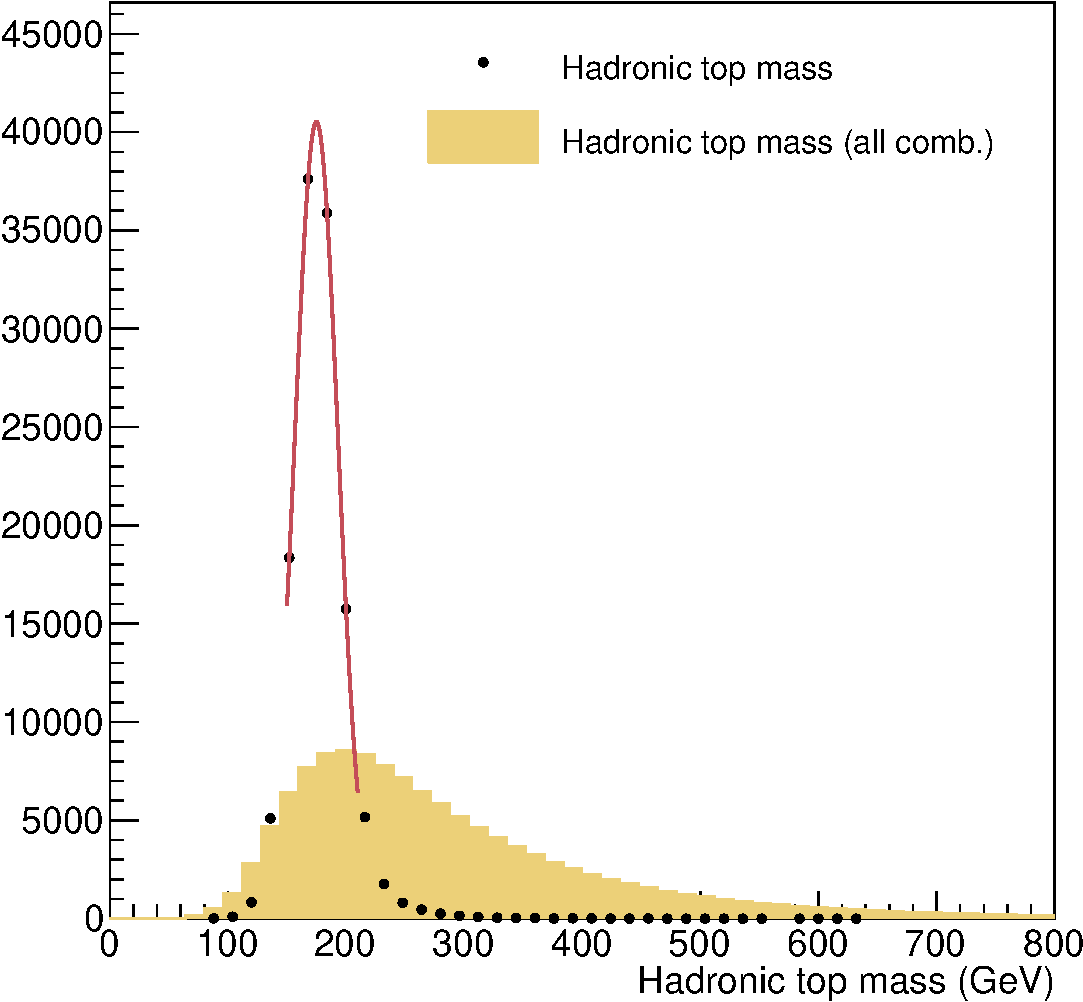
\includegraphics[width=0.41\textwidth]{chapitre6/figs/chi2/chi2_discrimant_combinations_hadronic_top_mass.pdf}} \qquad
    \subcaptionbox{}[0.41\textwidth]{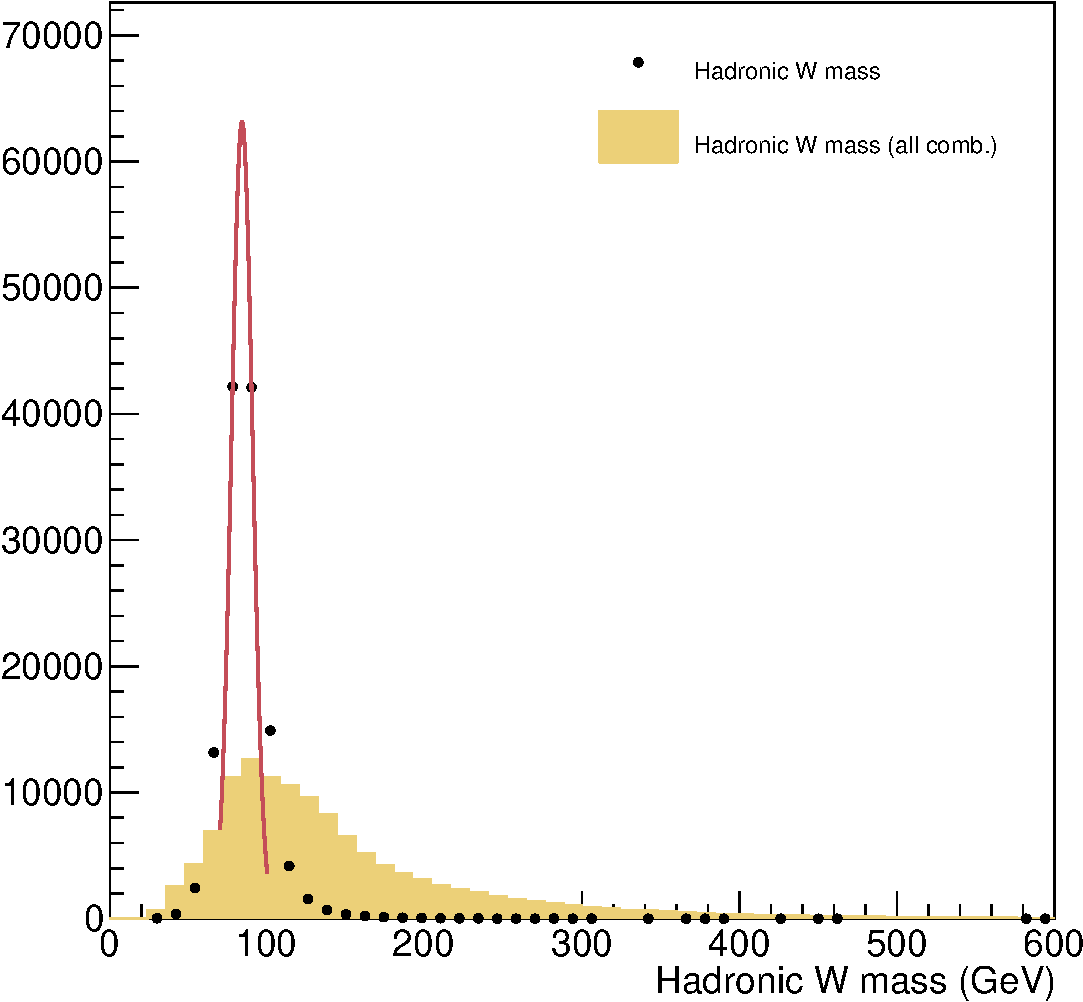
\includegraphics[width=0.41\textwidth]{chapitre6/figs/chi2/chi2_discrimant_combinations_w_mass.pdf}} \\
    \subcaptionbox{}[0.41\textwidth]{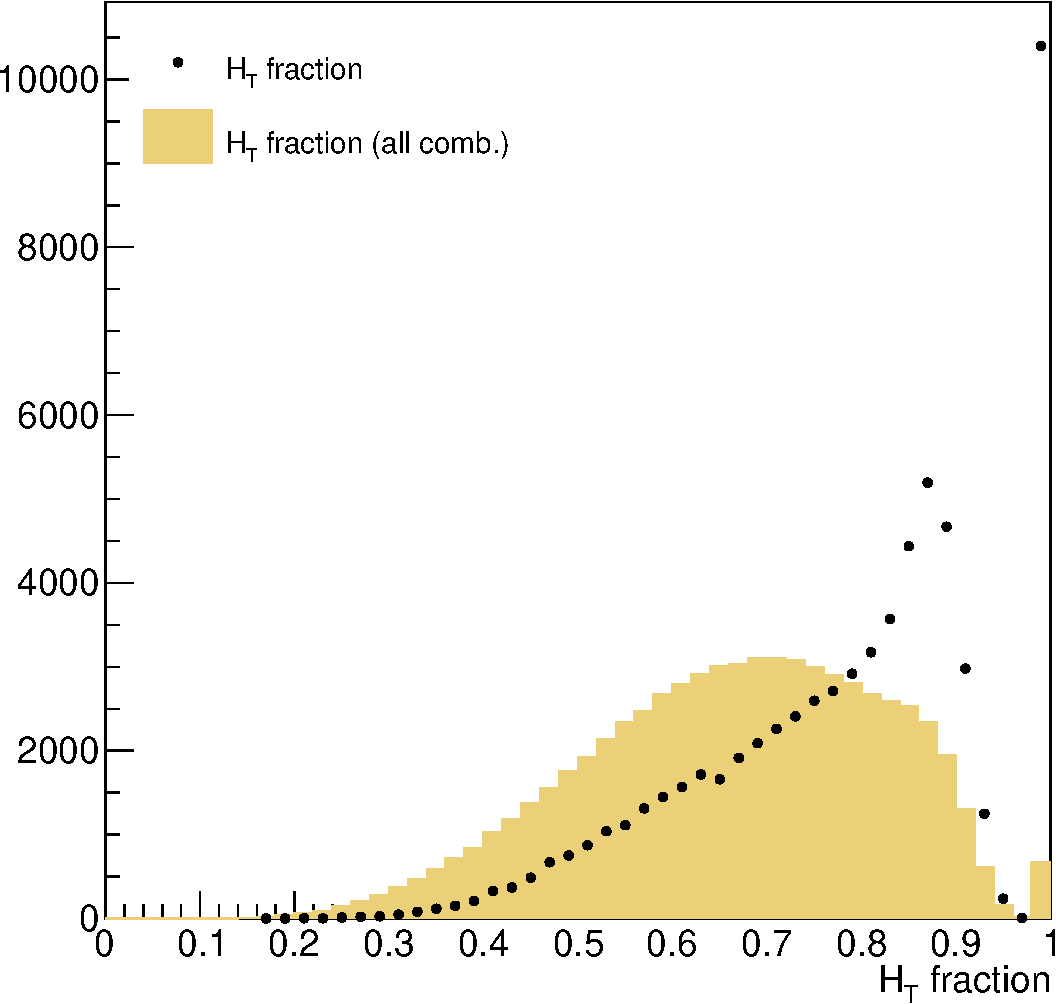
\includegraphics[width=0.41\textwidth]{chapitre6/figs/chi2/chi2_discrimant_combinations_ht_frac.pdf}}
    \caption{Distributions pour chaque discriminant du $\chi^2$. Les points noires correspondant aux valeurs calculées en utilisant les bonne combinaisons de jets, à comparer avec les valeurs calculées en utilisant toutes les combinaisons de jets (histogramme jaune). Une interpolation gaussienne est superposée afin d'extraire les valeurs de références ainsi que leurs erreurs. (a) $m_{\Ptop}^{\text{lept.}}$ semi-$\mu$. (b) $m_{\Ptop}^{\text{lept.}}$ semi-e. (c) $m_{\Ptop}^{\text{hadr.}}$. (d) $m_{\PW}^{\text{hadr.}}$. (e) $H_{T}^{\text{frac.}}$.}
    \label{fig:chi2_distributions}
\end{figure}

Afin d'extraire les valeurs de références des discriminants, on reconstruit l'événement \ttbar en utilisant uniquement la bonne association de jet. Cette bonne association est déterminée en utilisant la vérifié Monte Carlo. À chaque jet reconstruit (jet reco), on tente d'assigner un parton provenant de la désintégration \ttbar. Cette procédure d'assignation est réalisée en demandant que la distance entre le jet reco et le parton dans le plan $(\eta, \phi)$ ($\Delta R = \sqrt{\Delta \eta^2 + \Delta \phi^2}$) soit inférieure à $0.4$, et que la différence d'impulsion transverse ($\Delta p_T$) soit inférieure à \SI{300}{\%}. Dans le cas où aucune association ne peut être faite (\tilde \SI{60}{\%} des cas), l'événement n'est considéré ni pour les bonnes ni pour les mauvaises combinaisons.

\begin{table} \centering
    \begin{tabular}{@{}ccc@{}} \toprule
        Discriminant $x$& Valeur de référence $X_\text{MC}$ & Erreur ($\sigma_\text{MC}$) \\ \midrule
        $m_{\Ptop}^{\text{lept.}}$ (semi-e) & \SI{170.88}{\GeV} & \SI{17.29}{\GeV} \\
        $m_{\Ptop}^{\text{lept.}}$ (semi-$\mu$) & \SI{170.94}{\GeV} & \SI{17.36}{\GeV} \\
        $m_{\Ptop}^{\text{hadr.}}$ & \SI{175.16}{\GeV} & \SI{17.35}{\GeV} \\
        $m_{\PW}^{\text{hadr.}}$ & \SI{84.06}{\GeV} & \SI{10.12}{\GeV} \\
        $H_{T}^{\text{frac.}}$ & \num{1} & \num{0.15} \\ \bottomrule
    \end{tabular}
    \caption{Valeurs de références et erreurs pour chaque discriminant utilisé dans le calcul du $\chi^2$. Ces valeurs ont été déterminées sur des événements \ttbar simulés.}
    \label{tab:chi2_ref_values}
\end{table}

On évalue la valeur de chaque discriminant pour chaque bonne combinaison. On présente \cref{fig:chi2_distributions} les distributions de chaque discriminant. Les valeurs de références et les erreurs associées sont extraites grâce à une interpolation avec une fonction gaussienne (en rouge sur les figures). Seule la distribution de $H_T^\text{frac.}$ n'est pas gaussienne. Pour ce cas particulier, la valeur moyenne et la moyenne quadratique (RMS) de la distribution sont utilisées.


On présente \cref{tab:chi2_ref_values} les valeurs de références utilisées pour le calcul du $\chi^2$, avec leurs erreurs associées. Ces valeurs ont été déterminées sur des événements \ttbar simulés.

\bigskip

L'algorithme fonctionne de la façon suivante : on itère sur toutes les sous-ensembles de 4 jets de l'événement. Pour chaque sous-ensemble, on calcule pour chaque combinaison de jets la valeur du $\chi^2$. On retient au final la combinaison qui minimise le $\chi^2$. On peut voir \cref{fig:chi2_distribution} la distribution du $\chi^2$ pour toutes les combinaisons (bleu) et pour la bonne combinaison (rouge). On voit que choisir la valeur du $\chi^2$ la plus petite permet de sélectionner la bonne combinaison.

\begin{figure}[tbp] \centering
    \subcaptionbox{\label{fig:chi2_distribution}}[0.48\textwidth]{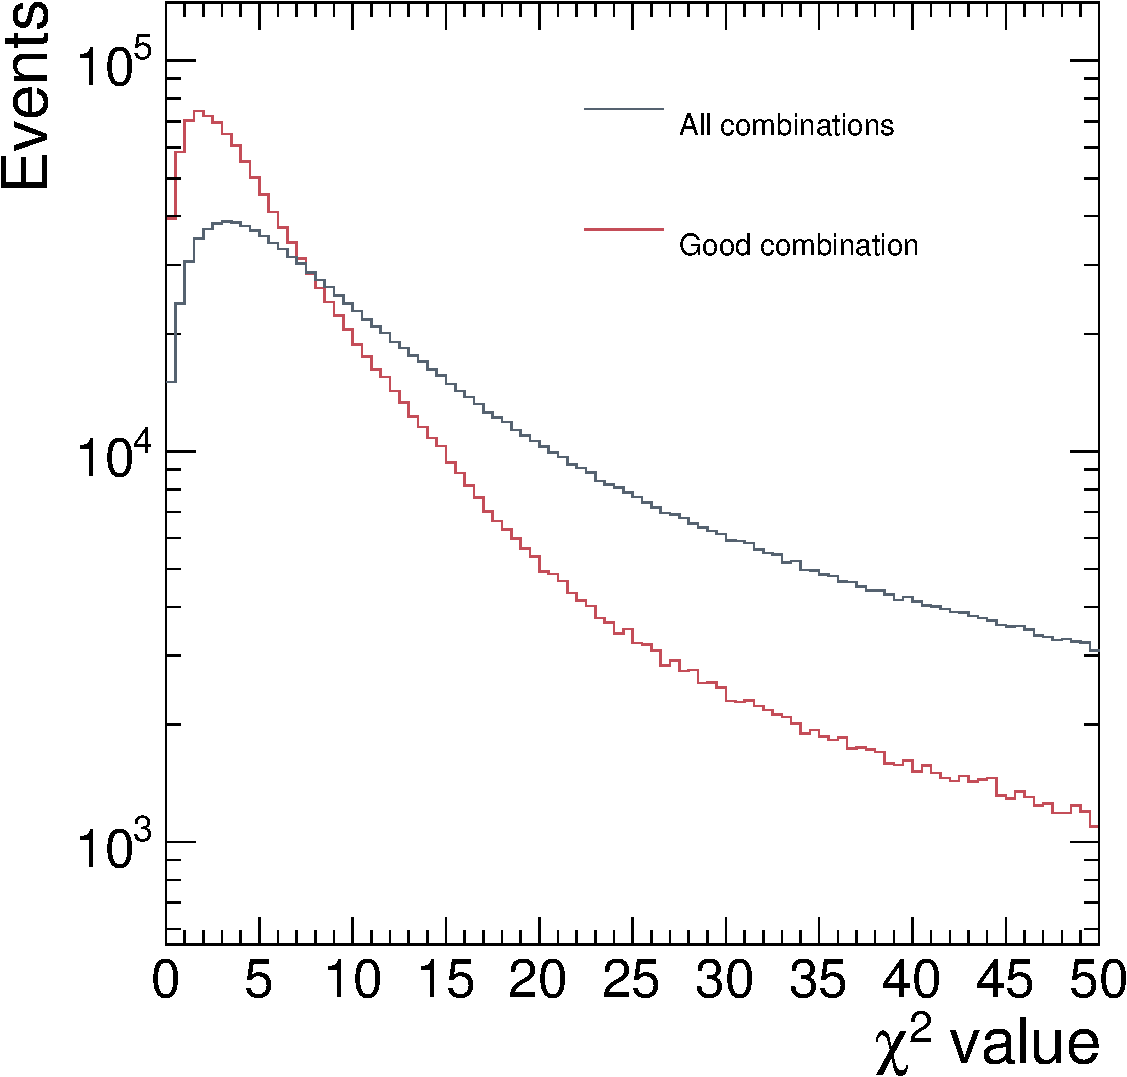
\includegraphics[width=0.48\textwidth]{chapitre6/figs/chi2/chi2_distribution.pdf}} \hfill
    \subcaptionbox{\label{fig:chi2_ptsyst}}[0.48\textwidth]{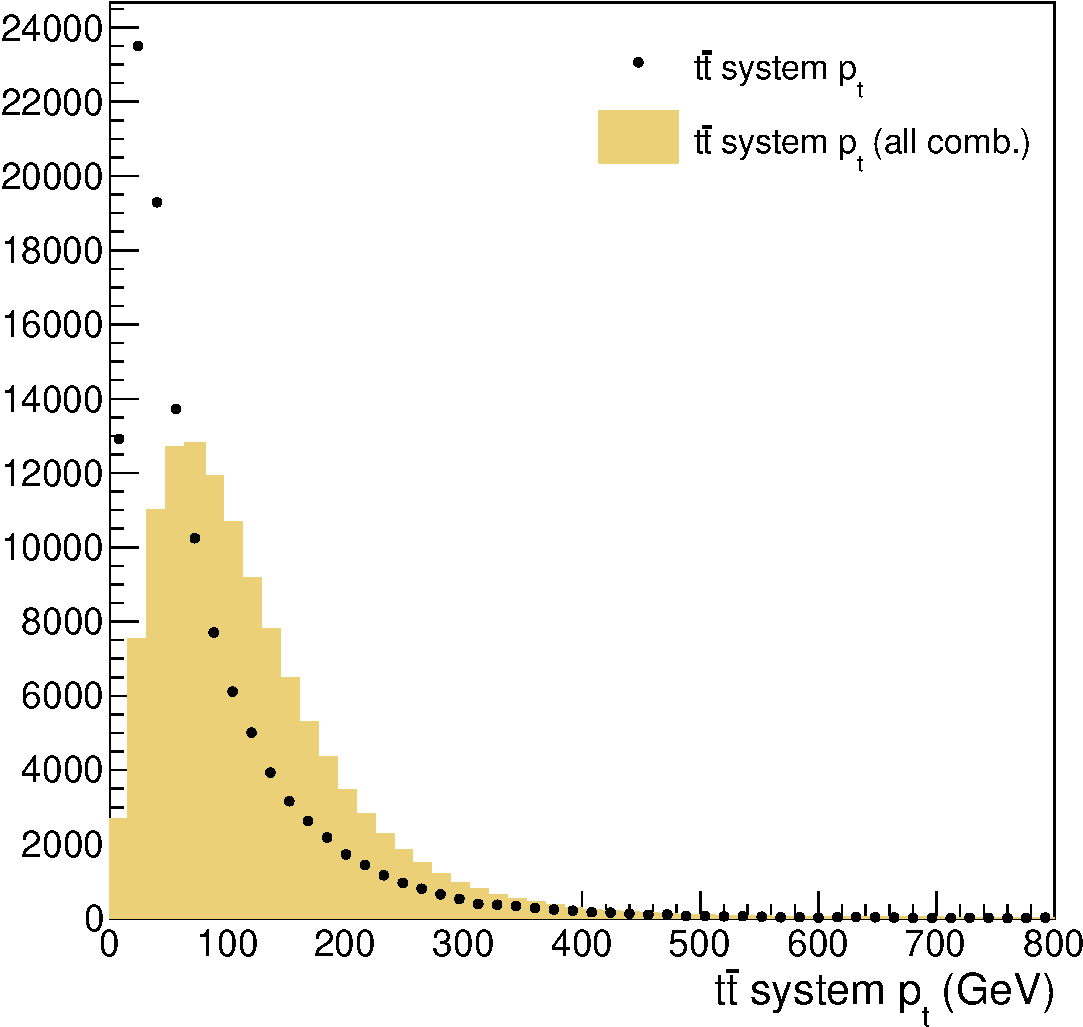
\includegraphics[width=0.48\textwidth]{chapitre6/figs/chi2/chi2_discrimant_combinations_pt_syst.pdf}}
    \caption{(\subref{fig:chi2_distribution}) Comparaison entre les distributions de $\chi^2$ pour toutes les combinaisons de jets (\textcolor{bleu_gris}{bleu}) et pour la bonne combinaison de jets (\textcolor{rouge_grandmere}{rouge}), réalisée à partir d'événements \ttbar simulées. (\subref{fig:chi2_ptsyst}) $p_T$ du système \ttbar pour les bonnes combinaisons ainsi que toutes les combinaisons.}
\end{figure}

Avant de pouvoir continuer la discussion, il est nécessaire de donner quelques définitions :

\begin{itemize}
    \item On parle d'\textbf{événement associable} s'il est possible d'associer à chaque parton de la désintégration \ttbar un jet reconstruit, selon la procédure détaillée ce-dessus.
    \item On parle d'\textbf{événement associé} si un événement est associable, et si l'algorithme de tri par $\chi^2$ à permis de choisir correctement les 4 bon jets provenant de la désintégration \ttbar. Pour cette classe d'événement, la position des jets n'est pas importante.
    \item Enfin, on parle d'\textbf{événement associé et bien placé} si un événement est associé, et si les 4 jets sélectionnés sont aussi bien placé, c'est-à-dire si le jet choisi pour être le jet \Pbottom leptonique est correct, etc.
\end{itemize}

Lorsque l'on reconstruit la masse invariante \ttbar, on reconstruit la masse invariante d'un système à 6 corps (voir \cref{eq:invariant_mass_tt}). La position des jets sélectionnés n'a au final aucune influence sur la valeur de la masse invariante. Seul importe le fait de choisir les 4 bons jets. On cherche donc à maximiser l'efficacité d'obtenir la bonne combinaison de jets. Pour cela, plusieurs études ont été faites afin de savoir si l'ajout d'un autre terme dans le $\chi^2$ permettrait d'améliorer cette efficacité. L'étude s'est concentré sur la possible d'ajouter le $p_T$ du système \ttbar comme variable discriminante. On peut voir \cref{fig:chi2_ptsyst} le pouvoir de discrimination d'une telle variable. Les résultats de cette étude sont présentés \cref{tab:chi2_study}, et on peut voir que le $\chi^2$ optimal est celui présenté \cref{eq:chi2}.

\begin{table}[h] \centering
    \begin{tabular}{@{}ccccc@{}} \toprule
        & sans $H_{T}^{\text{frac.}}$ ni $p_{T}^{\ttbar}$ & avec $p_{T}^{\ttbar}$ & avec $H_{T}^{\text{frac.}}$ & avec $H_{T}^{\text{frac.}}$ ni $p_{T}^{\ttbar}$ \\ \midrule
        $\epsilon_\text{associé}$ & \SI{76.80 \pm 0.37}{\%} & \SI{76.01 \pm 0.38}{\%} & \SI{80.01 \pm 0.35}{\%} & \SI{77.35 \pm 0.37}{\%} \\
        $\epsilon_\text{associé et bien placé}$ & \SI{23.44 \pm 0.37}{\%} & \SI{23.12 \pm 0.37}{\%} & \SI{24.47 \pm 0.38}{\%} & \SI{23.55 \pm 0.37}{\%} \\ \bottomrule
    \end{tabular}
    \caption{Efficacité d'obtenir un événement associé ($\epsilon_\text{associé}$) et un événement associé et bien placé ($\epsilon_\text{associé et bien placé}$) pour différentes configurations du $\chi^2$. La configuration optimale est celle utilisant uniquement le terme supplémentaire $H_{T}^{\text{frac.}}$.}
    \label{tab:chi2_study}
\end{table}

D'autres méthodes existent pour sélectionner la bonne combinaison de jets. La plus simple d'entre elle consiste à sélectionner les 4 jets de plus haute impulsion. On compare \cref{fig:chi2_vs_jets} les performances de l'algorithme de tri par $\chi^2$ par rapport à sélectionner les 4 jets de plus haute impulsion. On constate que l'algorithme de tri par $\chi^2$ est bien plus performant que le simple choix des 4 jets, avec une différence d'efficacité variant entre \tilde\SI{15}{\%} et \tilde\SI{30}{\%} en fonction de la masse invariante \ttbar générée.

\begin{figure}[tbp] \centering
    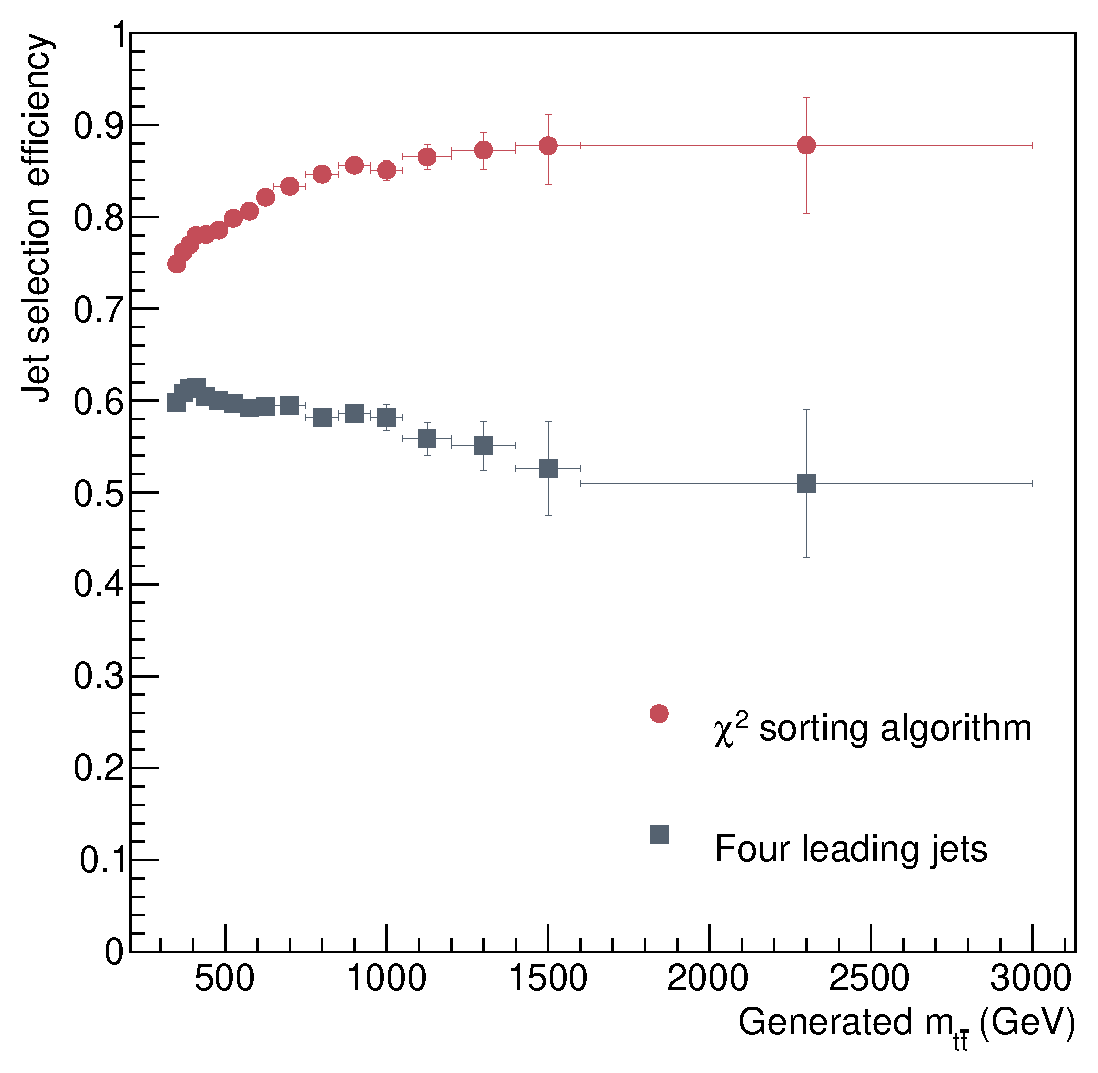
\includegraphics[width=0.50\textwidth]{chapitre6/figs/chi2/jet_selection_efficiency.pdf}
    \caption{Évolution de l'efficacité d'obtenir un événement associé en fonction de la masse invariante \ttbar généré pour l'algorithme de tri par $\chi^2$ (\textcolor{rouge_grandmere}{rouge}) ou en sélectionnant simplement les 4 jets de plus haute impulsions (\textcolor{bleu_gris}{bleu}).}
    \label{fig:chi2_vs_jets}
\end{figure}

\subsection{Algorithme de tri par MVA}

Des nombreuses variables rentrent en jeu lors du calcul de la masse invariante \ttbar. Une méthode simple pour les exploiter serait d'étendre le $\chi^2$ (\cref{eq:chi2}) pour ajouter autant de termes que nécessaire. Cela suppose néanmoins que les variables que l'on utilise comme discriminant soient gaussiennes, ce qui est le cas pour des distributions de masses invariantes, mais pas pour d'autres variables, telles que $\Delta \phi$ entre deux objets, ou l'impulsion transverse d'un autre objet.

Afin d'exploiter toutes les informations possibles pour discriminer entre bonnes et mauvaises combinaisons, une analyse multi-variée a été mise en place, utilisant comme algorithme les arbres de décisions boostés (BDT, \emph{Boosted Decision Tree}).

%Deux algorithmes différents sont comparées dans cette section : les arbres de décisions boostés (BDT, \emph{Boosted Decision Tree}) et les réseaux de neurones (NN, \emph{Neural Network}).

\subsubsection{Arbres de décisions boostés}

\begin{figure}[tbp] \centering
    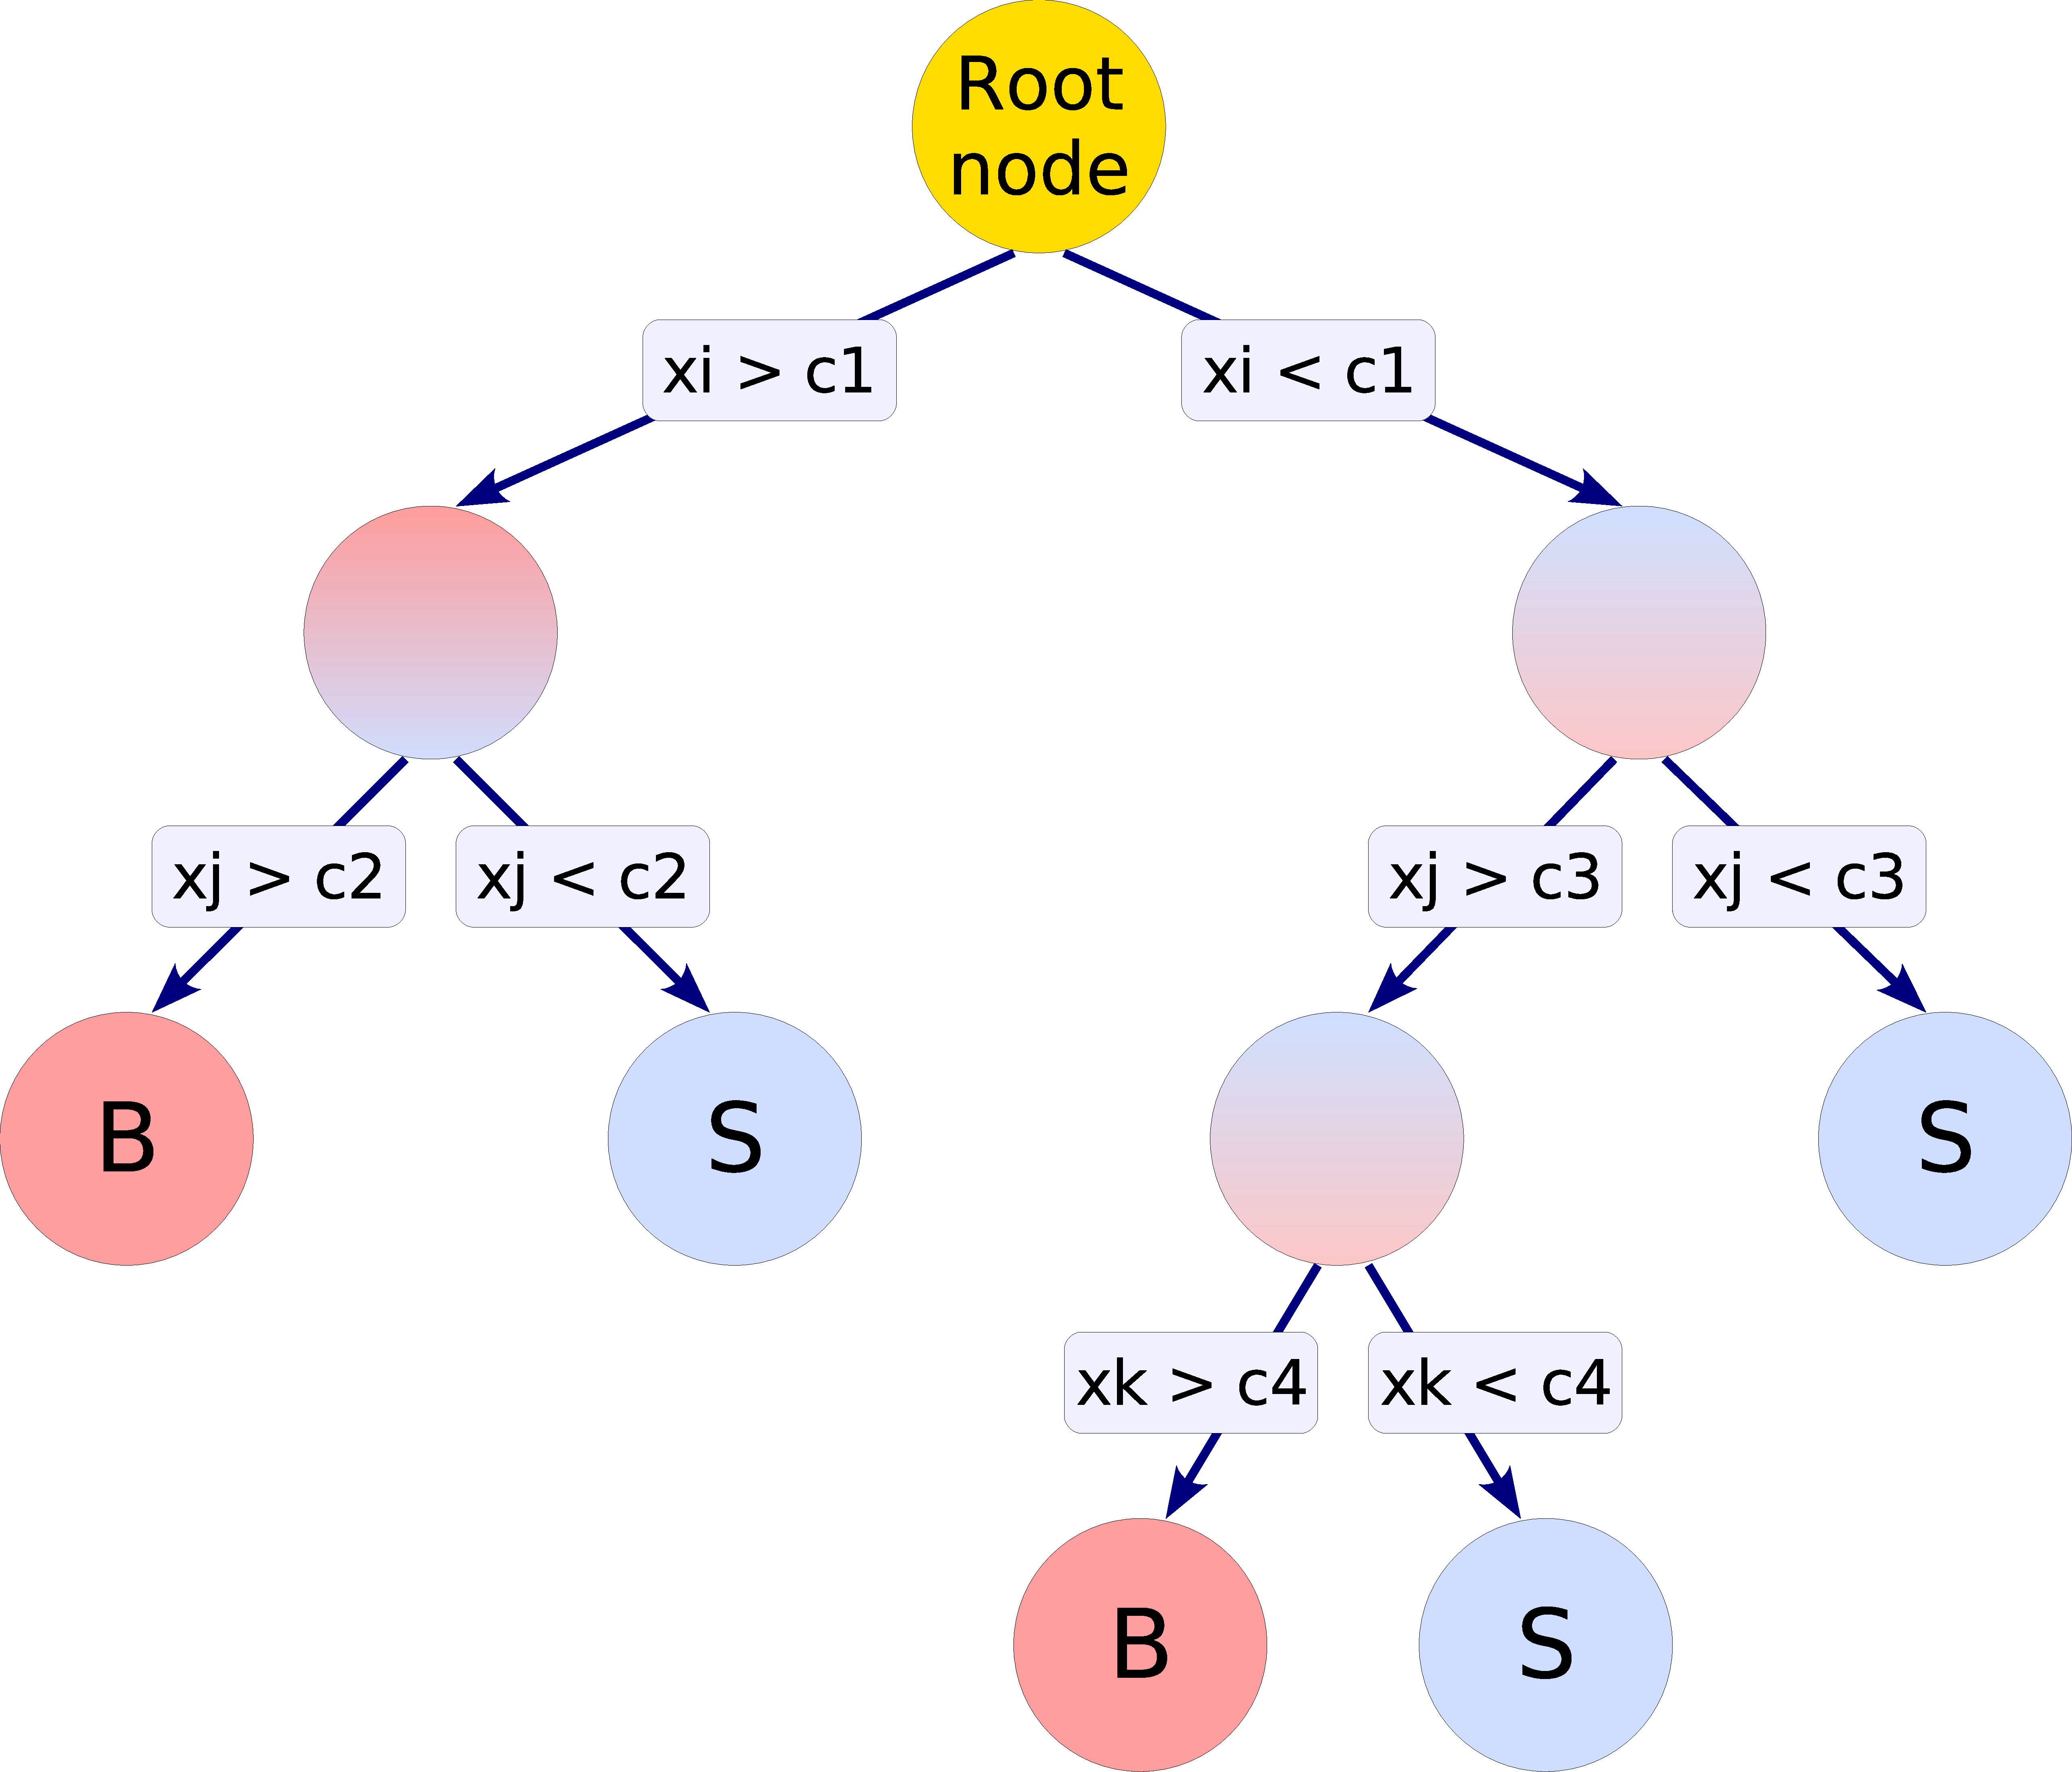
\includegraphics[width=0.55\textwidth]{chapitre6/figs/BDT.pdf}
    \caption{Vue schématique d'un arbre de décision. En commençant au nœud racine, une suite de sélections binaires sont appliquées en utilisant le discriminant $x_i$, qui peut varier ou non à chaque nœud de la sélection. A la fin de chaque branche de sélection, l'événement est classé comme "signal" (S) ou comme "fond" (B).}
    \label{fig:bdt}
\end{figure}

Un arbre de décision est un algorithme de classification des événements utilisant en entrée plusieurs variables, et qui permet en sortie de classer les événements en deux catégories distinct : "signal" ou "fond". L'algorithme commence au nœud racine, où une première coupure sur une variable $x_i$ est appliquée.Une deuxième coupure sur une variable $x_j$ est ensuite appliquée, qui dépend du résultat de la première coupure: on obtient ainsi 2 nouveaux noeuds. Cette procédure est répétée jusqu'à ce qu'une condition d'arrêt soit atteinte. L'événement est alors classé "signal" ou "fond". Un exemple d'arbre de décision est présenté \cref{fig:bdt}.

Afin de construire un tel arbre, une phase d'entrainement est nécessaire. Cette entrainement est réalisé à la fois sur des événements classés comme "signal" et sur des événements classés comme "fond". Un des principaux problèmes de cet algorithme est son instabilité vis-à-vis des fluctuations statistiques dans l'échantillon utilisé pour l'entrainement. Par exemple, si deux variables font preuves d'un pouvoir de discrimination similaire, une fluctuation statistique pourrait décider l'algorithme à utiliser la première variable au lieu de la deuxième.

Le problème est contourné en construisant une "forêt" d'arbres de décision. La classification d'un événement en "signal" ou "fond" est déterminée par le résultat majoritaire sur tous les arbres. L'entrainement de chaque arbre est réalisé sur le même échantillon. La seule différence vient de l'application d'un poids particulier à chaque événement : les événements mal classés durant l'entrainement de l'arbre de décision auront un poids plus grand lors de l'entrainement de l'arbre suivant. Cette technique est appelé \emph{boost} \citep{Freund1997119} et permet de stabiliser l'algorithme.

%\subsubsection{Réseau de neurones}
\fxnote{Réseau de neurones ?}

\subsubsection{Classification des événements \ttbar}

L'utilisation d'un BDT permet de classer un événement en deux catégories : "signal" ou "fond". Pour notre cas particulier, la catégorie "signal" correspond au choix de la bonne combinaison de jets, et "fond" aux mauvaises combinaisons. 14 variables rentrent dans la composition de nos MVA :

\begin{itemize}
    \item Variables à décider
\end{itemize}

\fxerror{Ajouter plots des variables et du BDT une fois finit d'entrainer}

\fxerror{Relancer extractor sur TT avec nouveaux BDT et comparer efficacités de de matching avec $\chi^2$}

% Une variable très discriminante, non incluse, est \mtt. Il n'est malheureusement pas possible d'utiliser cette variable, puisque l'on cherche à observer des déviations dans le spectre de masse invariante. Une telle déviation classerait notre événement dans la catégorie "fond".

\section{Ajustement cinématique}

Pour un événement \ttbar, les objets reconstruits (leptons, jets, ...) doivent vérifier certaines contraintes cinématiques, telle que la conservation de l'énergie ou reproduire la bonne masse invariante des particules. Néanmoins, l'impulsion et l'énergie des particules utilisées pour reconstruire l'événement \ttbar ne sont connues qu'avec une certaines incertitudes, liés à la résolution expérimentale, aux techniques de reconstruction, etc. Ces incertitudes peuvent conduire à un non-respect des contraintes d'un événement \ttbar.

\medskip

L'idée de l'ajustement cinématique est simple : faire varier les quantités physiques des objets sélectionnées, dans leurs incertitudes, afin de respecter au mieux les con\-traintes d'un événement \ttbar. On utilise pour cela la méthode des multiplicateurs de Lagrange afin de trouver les valeurs optimales des quantités physiques des particules sélectionnées sous diverses contraintes.

\bigskip

\begin{figure}[p] \centering
    \subcaptionbox{\label{fig:kinfit_matched_events}}[0.90\textwidth]{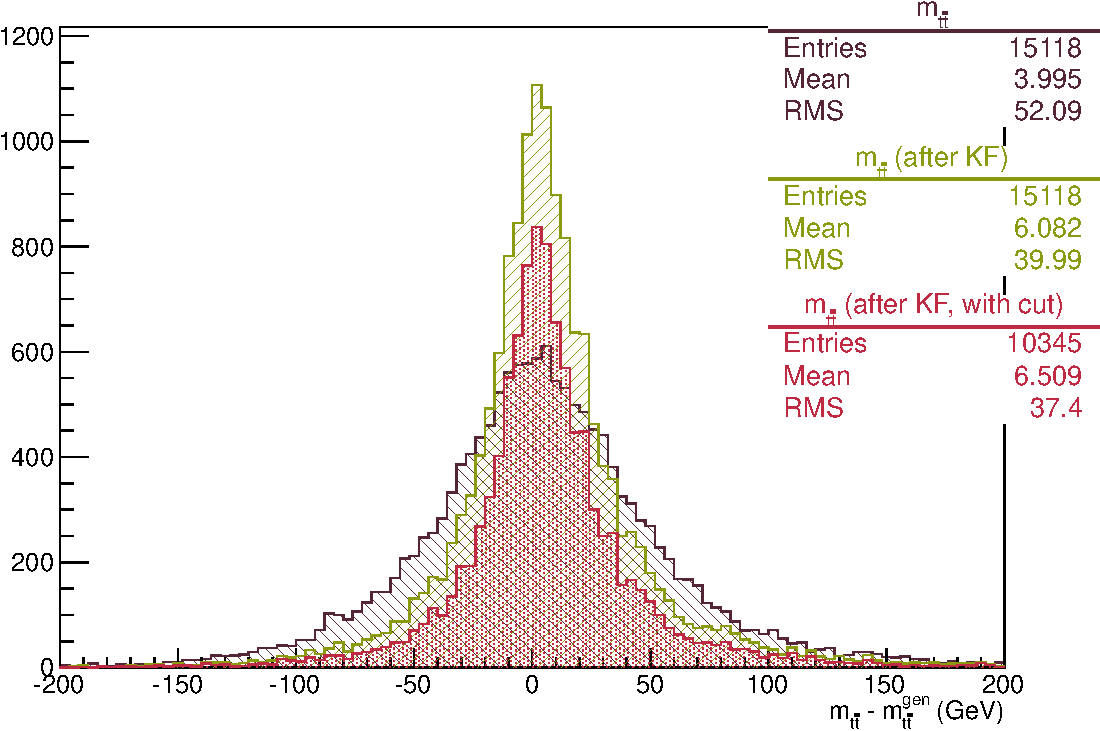
\includegraphics[width=0.90\textwidth]{chapitre6/figs/kinfit/mtt_resolution_with_kinfit_2011_resolutions_good_solutions_on_TTbar.pdf}} \\
    \subcaptionbox{\label{fig:kinfit_all_events}}[0.90\textwidth]{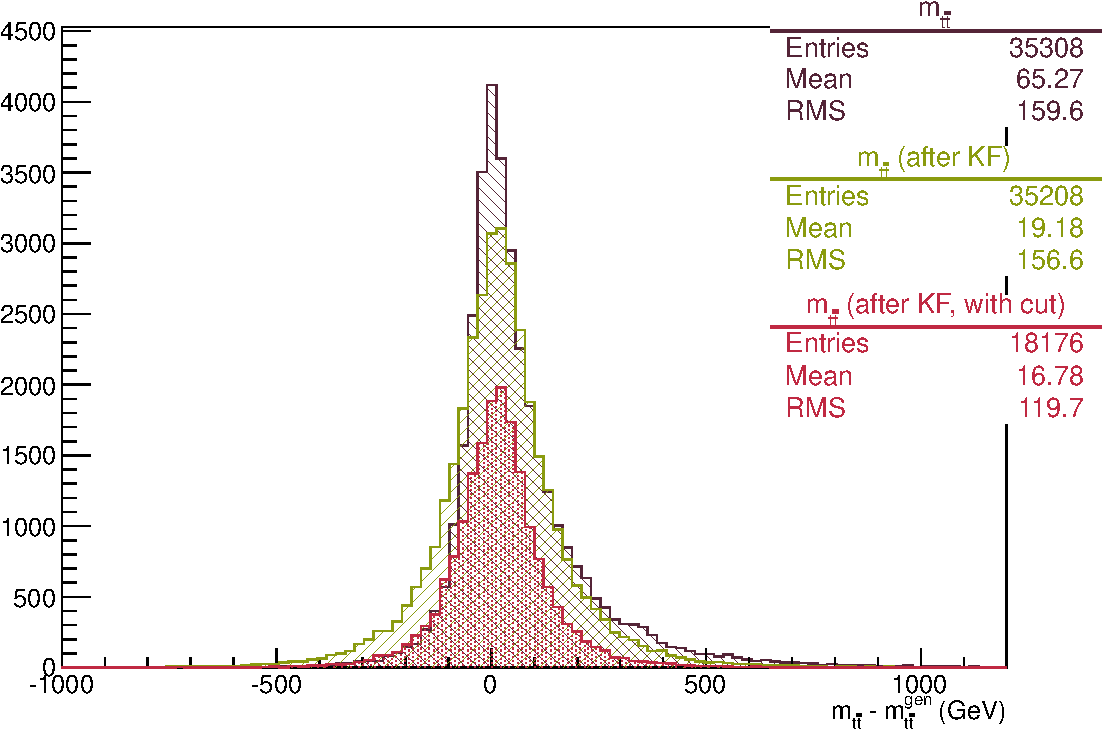
\includegraphics[width=0.90\textwidth]{chapitre6/figs/kinfit/mtt_resolution_with_kinfit_2011_resolutions_on_TTbar.pdf}}
    \caption{Résolution sur la masse invariante \mtt sans ajustement cinématique (\textcolor{violet}{violet}), après ajustement cinématique (\textcolor{vert}{vert}) et après ajustement cinématique et une coupure $p > 0.2$ (\textcolor{rouge_grandmere}{rouge}). Les distributions ont été obtenues avec des événements \ttbar simulés, en utilisant la bonne combinaison de jets (\subref{fig:kinfit_matched_events}) et avec tous les événements (\subref{fig:kinfit_all_events}).}
    \label{fig:kinfit_ttbar}
\end{figure}

On utilise l'ajustement cinématique en sortie de l'algorithme de tri par $\chi^2$ : les particules provenant de la désintégration des paires \ttbar sont déjà sélectionnées. L'ajustement cinématique est donc utilisé uniquement pour ajuster au mieux les contraintes, et non pas pour le choix des bonnes combinaisons de jets. Les contraintes utilisées dans l'algorithme sont les suivantes :
\begin{itemize}
    \item La masse invariante des deux jets légers doit être égale à la masse du boson \PW.
    \item La masse invariante du neutrino, du lepton ainsi que du jet \Pbottom leptonique doit être égale à la masse du quark top.
    \item La masse invariante des deux jets légers ainsi que du jet \Pbottom hadronique doit être égale à la masse du quark top.
\end{itemize}

L'effet de l'ajustement cinématique sur la résolution de la masse invariante est présenté \cref{fig:kinfit_ttbar} pour des événements \ttbar simulés. Afin d'améliorer les performances de l'ajustement cinématique, une coupure supplémentaire est réalisée sur la valeur de sortie $p$ de l'algorithme, qui définie la qualité de l'ajustement. On demande $p > 0.2$ (courbe \textcolor{rouge_grandmere}{rouge} sur les distributions des figures \ref{fig:kinfit_ttbar}).

% Pour chaque objet physique, on définit le lagrangien
% \begin{align*}
%   L(\vec{x}, \vec{\lambda}) &= \phi(\vec{x}) + \vec{\lambda} \cdot \left( \psi(\vec{x}) - c \right)
% \end{align*}
% où 

% Résoudre
% \begin{align*}
%   \nabla_{\vec{x}, \vec{\lambda}} L(\vec{x}, \vec{\lambda}) &= 0
% \end{align*}

\bigskip

L'utilisation de l'ajustement cinématique permet d'améliorer la résolution sur la masse invariante d'environ \SI{25}{\%} sur des événements associés et de près de \SI{40}{\%} en utilisant tous les événements. Cependant, ce gain en résolution est contrebalancé par une perte d'efficacité de sélection d'environ \SI{45}{\%} en utilisant uniquement des événements associés, et \tilde\SI{95}{\%} en utilisant tous les événements. Si l'on ne coupe pas sur $p$, l'efficacité reste constante, mais le gain en efficacité n'est plus que de \tilde\SI{5}{\%}.

\bigskip

On verra dans le \cref{chap:zprime} que ces bons résultats sur des événements \ttbar du Modèle Standard ne présagent pas de bonnes performances pour des événements \ttbar produit par de la nouvelle physique. En effet, l'utilisation de l'ajustement cinématique dégrade la résolution sur \mtt lorsqu'il est utilisé sur autre chose que des événements \ttbar Modèle Standard. Une étude plus détaillée sera présentée dans le prochain chapitre, mais on peut déjà dire que l'ajustement cinématique n'a finalement pas été utilisé pour reconstruire la masse invariante \ttbar.

\section{Conclusion}

Comme on a pu le voir tout au long de ce chapitre, deux étapes sont nécessaires pour reconstruire la masse invariante \ttbar. Dans un premier temps, il est nécessaire de choisir correctement les jets provenant de la désintégration des quarks top, et non pas des jets provenant du \pu ou de radiations. Pour cela, plusieurs algorithmes existent, dont deux ont été détaillés dans ce chapitre. Une fois les jets sélectionnés, il reste encore à reconstruire le composante longitudinale de l'impulsion du neutrino, ce qui permet d'évaluer correctement l'énergie de ce neutrino.

Toutes ces techniques sont utilisées avec succès dans les analyses de recherche de nouvelles physiques, qui sont les sujets des \cref{chap:zprime,chap:higgs}.